\chapter{Literature Review}
\label{chap:literature-review}

\section{Introduction}
\label{sec:lr-introduction}

Cross-silo federated learning (FL) changes where model fitting occurs: each institution computes with its own records, while a coordinating process combines institution-level contributions into a shared model \cite{mcmahan2017fedavg}. For healthcare consortia, this arrangement avoids constructing a single repository of raw clinical records, but it does not remove the need for security controls. Shared updates may expose properties of training examples, a participating institution may deliberately corrupt the learning process, and cryptographic protection can make every communication round substantially more expensive \cite{shokri2017membership,zhu2019dlg,bagdasaryan2020backdoor}. Accordingly, this review examines protected healthcare FL as an interaction among learning, privacy, communication, adversarial robustness, and institutional governance.

The review covers literature published from January 2016 to August 2026, while retaining earlier foundational work where it defines a concept used by the proposed framework. Peer-reviewed journal articles and conference papers form the primary evidence base. Standards, dataset records, and official software or system descriptions are included only when they clarify an implementation or evaluation choice. The scope combines eight connected themes: cross-silo FL, optimization under institutional heterogeneity, differential privacy (DP), homomorphic encryption and secure aggregation, communication-efficient learning, privacy and poisoning attacks, Byzantine-robust aggregation, and permissioned audit and key governance. Healthcare studies are emphasized, but influential general FL and cryptography papers are included because many of the relevant security mechanisms were first evaluated outside clinical settings.

The review has three aims. First, it explains the theoretical models required to reason about utility, privacy, communication, and trust in multi-institutional learning. Second, it synthesizes empirical evidence concerning healthcare FL and the principal privacy-preserving and attack-resistant methods. Third, it identifies the unresolved integration and evaluation gaps that motivate the hybrid framework developed in this thesis. Accordingly, a reported result is interpreted together with its dataset, adversary model, visibility assumptions, and evaluation protocol. Results obtained on different datasets are not treated as direct evidence that one method is superior to another.

The search was conducted across IEEE Xplore, ACM Digital Library, PubMed, Scopus-indexed publisher collections, Web of Science-indexed sources, SpringerLink, ScienceDirect, the Proceedings of Machine Learning Research, NeurIPS proceedings, and USENIX proceedings. Searches combined terms such as \textit{federated learning}, \textit{cross-silo healthcare}, \textit{differential privacy}, \textit{CKKS}, \textit{secure aggregation}, \textit{gradient compression}, \textit{membership inference}, \textit{gradient reconstruction}, \textit{model poisoning}, \textit{Byzantine aggregation}, \textit{threshold decryption}, and \textit{permissioned blockchain}. Studies were included when they presented a relevant method, system, dataset, attack, or reproducible empirical analysis. Non-technical opinion pieces, duplicate versions, papers without enough methodological detail, and studies unrelated to collaborative learning were excluded. In a lightweight PRISMA-style flow, records were identified by database and backward-reference searches, deduplicated, screened by title and abstract, assessed in full text for relevance, and then grouped by technical function. Because this is a focused narrative review rather than a registered systematic review, the process is reported transparently without claiming PRISMA certification.

The remainder of the chapter follows the university's required structure. Section~\ref{sec:theory} develops the theoretical background and existing models. Section~\ref{sec:related-studies} organizes related studies by research theme and critically examines the closest anchor papers. Section~\ref{sec:comparative-analysis} compares the principal approaches using common criteria. Section~\ref{sec:research-gaps} consolidates the resulting gaps and maps them to the objectives of this thesis.

\section{Theoretical Background and Existing Models}
\label{sec:theory}

\subsection{Cross-Silo Federated Learning}

In centralized learning, a coordinator holds the entire training dataset and minimizes an empirical loss over all records. Cross-silo FL instead distributes those records among a relatively small number of stable organizations, such as hospitals. Let hospital $k$ hold dataset $D_k$ containing $n_k$ records, and let $n=\sum_{k=1}^{K} n_k$. A common global objective is
\begin{equation}
    \min_{\mathbf{w}} F(\mathbf{w})
    = \sum_{k=1}^{K}\frac{n_k}{n}F_k(\mathbf{w}),
    \qquad
    F_k(\mathbf{w})=\frac{1}{n_k}\sum_{i\in D_k}\ell(\mathbf{w};x_i,y_i),
    \label{eq:fl-objective}
\end{equation}
where $\mathbf{w}$ denotes the model parameters and $\ell$ is the task loss. In a FedAvg round, selected institutions receive the current parameter vector, update it through local stochastic optimization, and return their changes for sample-size-weighted combination \cite{mcmahan2017fedavg}. Performing several computations before this exchange can reduce the number of synchronizations required relative to a method that communicates after every gradient step.

Healthcare deployments differ from the large, intermittent cross-device setting that motivated early FL. Hospitals are normally identifiable, continuously governed, and connected through institutional infrastructure. They also exhibit non-independent and non-identically distributed (non-IID) data because patient populations, equipment, clinical pathways, coding practices, and label prevalence vary by site. Collaborative medical studies have demonstrated that FL can approach centralized training without moving source records, including multi-institutional brain-tumour segmentation and COVID-19 outcome prediction \cite{sheller2020federated,dayan2021federated}. However, these results also show that local retention is only the first layer of protection: an operational system must define who may participate, which updates are accepted, how secrets are governed, and how actions are audited.

\subsection{Federated Optimization under Heterogeneity}

FedAvg can drift when local objectives differ or clients perform unequal amounts of local computation. FedProx adds the proximal penalty $\frac{\mu}{2}\lVert\mathbf{w}-\mathbf{w}_t\rVert_2^2$ to each local objective, discouraging an institution's model from moving too far from the current global model \cite{li2020fedprox}. SCAFFOLD estimates server and client control variates to correct the gradient drift caused by heterogeneous data \cite{karimireddy2020scaffold}. FedNova addresses a different inconsistency: when clients perform different numbers of local steps, conventional weighted averaging can optimize a distorted objective, so FedNova normalizes local updates before aggregation \cite{wang2020fednova}. Adaptive server optimizers such as FedAdam and FedYogi apply coordinate-wise learning-rate adaptation to the aggregated update and can improve convergence without altering client data ownership \cite{reddi2021adaptive}.

These methods improve optimization, not confidentiality or adversarial robustness. Their value in this thesis is therefore twofold. They establish strong utility baselines under hospital heterogeneity, and they separate optimization failure from security failure. If a protected method loses predictive performance, comparison with FedProx, SCAFFOLD, and FedNova helps determine whether the loss comes from non-IID training, privacy noise, compression, or an attack defence.

\subsection{Differential Privacy}

Following the neighbouring-dataset formulation of differential privacy, two inputs differ in one protected unit, and the output distributions produced from those inputs must remain close \cite{dwork2006calibrating}. Formally, a randomized mechanism $\mathcal{M}$ satisfies $(\epsilon,\delta)$-differential privacy when every measurable output set $S$ obeys
\begin{equation}
    \Pr[\mathcal{M}(D)\in S]
    \leq e^{\epsilon}\Pr[\mathcal{M}(D')\in S]+\delta.
    \label{eq:dp-definition}
\end{equation}
Here, a smaller $\epsilon$ gives a tighter bound, and $\delta$ permits a limited probability of an outcome not covered by the pure-DP term. DP-SGD operationalizes this definition for iterative learning by bounding each example's gradient contribution and perturbing the aggregate with calibrated noise \cite{abadi2016deep}. A privacy accountant then composes the loss incurred across the complete sequence of training steps.

The protected unit must be stated explicitly. Record-level DP limits the influence of one patient record, whereas client-level DP limits the influence of an entire institution. In cross-silo healthcare, client-level protection can require severe noise because the number of hospitals is small, while record-level DP may be appropriate when the research question concerns patient participation. Private adaptive clipping estimates a clipping quantile without exposing the distribution of update norms and is compatible with secure aggregation \cite{andrew2021adaptive}. Yet DP introduces a genuine utility--privacy trade-off: stronger clipping and larger noise can reduce discrimination, calibration, or minority-group performance. Consequently, a privacy claim requires the adjacency definition, clipping rule, sampling model, accountant, $\epsilon$, $\delta$, and secure random-number source, not merely the statement that noise was added.

\subsection{Homomorphic Encryption, Secure Aggregation, and Threshold Governance}

Homomorphic encryption permits computation on ciphertexts. Gentry's construction established the feasibility of fully homomorphic encryption \cite{gentry2009fully}, while the CKKS scheme made approximate arithmetic over packed real or complex values practical for numerical workloads \cite{cheon2017homomorphic}. In an FL round, each hospital can encode and encrypt an update, after which the server adds the ciphertexts and obtains an encryption of their sum. The ciphertext operations do not expose the individual plaintext updates to an honest-but-curious aggregator.

CKKS is approximate rather than exact. Its parameters determine the polynomial modulus degree, coefficient modulus chain, scale, packing capacity, security level, precision, and runtime. Packing many coordinates into each ciphertext amortizes metadata and cryptographic overhead. It also creates a systems constraint: compression only reduces encrypted wire traffic when the retained coordinates share an agreed layout that can be packed compactly. Client-specific sparse supports must otherwise reveal indices or be encoded back into a dense vector, erasing the claimed ciphertext saving.

Secure aggregation is a related but distinct primitive. The protocol of Bonawitz et al. lets a server learn an aggregate while hiding each individual contribution and tolerating client dropouts \cite{bonawitz2017practical}. FLDP later combined distributed DP noise with an LWE-based malicious-secure aggregation protocol and reduced communication expansion relative to the secure-aggregation baseline evaluated in that work \cite{stevens2022fldp}. Both approaches protect update visibility, but neither makes a poisoned update benign. Once aggregation reveals only a sum, defences that require inspection of each plaintext vector may become incompatible with the privacy mechanism.

Threshold governance distributes decryption authority. Instead of allowing one trusted party to hold a complete secret key, a $t$-of-$n$ policy requires a threshold of custodians to authorize or construct a decryption. Multiparty homomorphic encryption extends this idea to collaborative computation and can remain private even when all but one party are semi-honest, subject to its stated protocol assumptions \cite{mouchet2021multiparty}. POSEIDON demonstrates multiparty lattice-based neural-network training without a trusted party, but evaluates a passive adversary and a computationally intensive setting rather than poisoning-resistant clinical FL \cite{sav2021poseidon}. Threshold authorization therefore reduces single-key custody risk, but it does not by itself prove that the decrypted aggregate is correct, that a custodian runs attested code, or that a malicious quorum cannot authorize an improper operation.

\subsection{Communication-Efficient Federated Learning}

Communication can dominate cross-institutional training because modern models contain millions of parameters and protected updates may expand after encryption. Common techniques include quantization, random sparsification, Top-$k$ selection, structured sparsity, and error feedback. Error feedback stores the compression residual and reinjects it in later rounds, reducing the long-term bias of aggressive compressors. Fed-EF analyzes this mechanism under heterogeneous data and partial participation, while also identifying stale residuals as a challenge when clients participate intermittently \cite{li2023fedef}.

Compression and privacy can interact constructively. SoteriaFL develops a local-DP framework for general shifted compression operators and studies the resulting privacy--communication--optimization trade-off \cite{li2022soteriafl}. Chen et al. show that partial communication can amplify privacy for distributed estimation under central or shuffle models \cite{chen2023privacycompression}. PREAMBLE provides privacy-preserving aggregation of block-sparse vectors through a two-server construction based on Prio and distributed point functions \cite{asi2025preamble}. However, these results cannot be transferred automatically to CKKS-based cross-silo learning. A theoretically sparse update may still occupy dense ciphertexts, and local DP may have a different utility profile from record-level central DP composed with protected aggregation.

The proposed framework uses ciphertext-aligned adaptive block compression (CAABC-FL). Its conceptual distinction is that the selected support is organized into common contiguous blocks before encryption, so logical sparsity corresponds to fewer serialized CKKS ciphertexts. Error feedback retains information omitted in one round, while validation-driven adaptation changes the block budget only using non-test evidence. This design treats the compressor, ciphertext layout, and evaluation protocol as one mechanism rather than measuring plaintext sparsity and assuming an equivalent network saving.

\subsection{Threat Model: Privacy, Integrity, and Availability}

An honest-but-curious aggregation server follows the protocol but attempts to infer private information from messages it legitimately receives. Membership-inference attacks test whether a record participated in training \cite{shokri2017membership}; stronger likelihood-ratio attacks demonstrate that average-case attack accuracy can conceal meaningful leakage at low false-positive rates \cite{carlini2022membership}. Gradient-reconstruction attacks optimize a candidate input so that its gradient matches an observed update. Deep Leakage from Gradients established the basic attack, and later work showed that recognizable reconstructions may remain possible from averaged gradients \cite{zhu2019dlg,geiping2020inverting}. These findings explain why transport encryption alone is insufficient: once a server receives a plaintext update, the server can attack it after transport decryption.

Integrity attacks have a different objective. A Byzantine or malicious institution may upload arbitrary model parameters, scale its update, flip signs or labels, create a backdoor, or coordinate with Sybil participants. Model-replacement attacks demonstrate that a single participant can implant a backdoor by exploiting the linear aggregation rule \cite{bagdasaryan2020backdoor}. Fang et al. further show that local model poisoning can be constructed against Byzantine-robust aggregation rules rather than merely against averaging \cite{fang2020local}. Longitudinal attackers can behave normally until reputation is accumulated and then activate a sleeper or adaptive attack. Therefore, robustness evaluation should vary attacker fraction, strength, duration, collusion, and knowledge, and should report both utility and availability failures such as excessive rollback.

\subsection{Robust Aggregation and Trust Management}

Krum chooses the update whose distances to neighbouring updates are most consistent with an assumed bound on Byzantine clients \cite{blanchard2017krum}. Coordinate-wise median and trimmed mean aggregate each parameter robustly and can achieve strong statistical rates under their assumptions \cite{yin2018byzantine}. Robust Federated Aggregation (RFA) replaces the mean with a geometric median and computes it using a smoothed Weiszfeld procedure \cite{pillutla2022robust}. FLTrust compares each client update with a server update computed on a small trusted root dataset and uses the resulting trust score in aggregation \cite{cao2021fltrust}. FLAME clusters updates, clips anomalous norms, and adds noise to mitigate backdoors \cite{nguyen2022flame}.

These defences are valuable controls, but most require access to individual plaintext updates or a clean reference dataset. That requirement conflicts with sum-only CKKS aggregation. Moreover, their theoretical guarantees depend on restrictions concerning attacker fraction, distributional similarity, or bounded deviation. A validation, rollback, and reputation layer offers a different control point: an independently evaluated candidate global model can be rejected if it violates a pre-committed acceptance rule, and the event can influence an institution's future reputation. This protects the released global state and preserves an evidence trail, but it can reduce availability and cannot identify every stealthy attacker. It should therefore be described as an empirical gate for specified attacks, not as a universal Byzantine proof.

\subsection{Permissioned Ledgers and Independent Verification}

A permissioned ledger can bind institutional identities to signed events, preserve ordered hashes of models and decisions, and make later alteration evident. Hyperledger Fabric separates execution, ordering, and validation and supports identity-aware policies suitable for organizational consortia \cite{androulaki2018hyperledger}. Blockchain-based FL designs such as BlockFL replace or supplement centralized coordination with consensus, but their latency analysis shows that block generation and consensus add to the end-to-end round time \cite{kim2020blockfl}.

Ledger immutability is often overstated. A ledger can prove that a particular hash, signature, or decision was recorded; it cannot prove that the associated model was clinically valid, that encryption was configured securely, or that off-chain data were truthful. Similarly, an aggregation verifier can recompute commitments, weights, and aggregate relationships independently, but only for the values and protocol transcript it can observe. The defensible role of the ledger is therefore accountability and tamper evidence. Privacy, model integrity, decryption governance, and semantic correctness still require separate controls.

\section{Related Studies}
\label{sec:related-studies}

The related literature did not develop as one continuous line of work. Healthcare demonstrations, formal privacy, encrypted computation, communication reduction, and poisoning defence advanced through partly separate research communities. Figure~\ref{fig:related-work-timeline} places representative milestones from these streams on one timeline and uses a distinct final marker for the present thesis in 2026. It is a thematic chronology rather than a claim that each later study superseded the earlier ones; the studies use different datasets, threat models, and evaluation units.

\begin{figure}[htbp]
\centering
\resizebox{\textwidth}{!}{%
\begin{tikzpicture}[
    font=\small,
    milestone/.style={draw, rounded corners=2pt, align=center, text width=2.65cm, minimum height=12mm, fill=blue!7},
    year/.style={draw, circle, fill=blue!70, text=white, minimum size=9mm, inner sep=1pt},
    stem/.style={draw=gray!70, line width=0.8pt},
    axis/.style={-{Latex[length=2.2mm]}, line width=1.1pt, draw=gray!80}
]
\draw[axis] (-0.6,0) -- (17.6,0);

\node[year] (y2017) at (0,0) {2017};
\node[milestone, above=7mm of y2017] {FedAvg establishes\\iterative federated\\optimization};

\node[year] (y2020) at (2.45,0) {2020};
\node[milestone, below=7mm of y2020] {Natural multi-hospital\\healthcare FL\\demonstration};

\node[year] (y2021) at (4.90,0) {2021};
\node[milestone, above=7mm of y2021] {EXAM multi-site study;\\FAMHE and POSEIDON\\protected computation};

\node[year] (y2022) at (7.35,0) {2022};
\node[milestone, below=7mm of y2022] {FLamby healthcare\\benchmark; FLDP and\\SoteriaFL integration};

\node[year] (y2023) at (9.80,0) {2023};
\node[milestone, above=7mm of y2023] {Fed-EF analysis of\\biased compression and\\error feedback};

\node[year] (y2024) at (12.25,0) {2024};
\node[milestone, below=7mm of y2024] {DDFed encrypted\\anomaly detection;\\privacy--fairness studies};

\node[year] (y2025) at (14.70,0) {2025};
\node[milestone, above=7mm of y2025] {DP-BREM+ robustness;\\PREAMBLE private\\block-sparse aggregation};

\node[year, fill=teal!70!black] (y2026) at (17.15,0) {2026};
\node[milestone, below=7mm of y2026, fill=teal!10, draw=teal!70!black]
{Present thesis:\\CAABC-FL and governed\\end-to-end evaluation};

\draw[stem] (y2017.north) -- ++(0,0.7);
\draw[stem] (y2020.south) -- ++(0,-0.7);
\draw[stem] (y2021.north) -- ++(0,0.7);
\draw[stem] (y2022.south) -- ++(0,-0.7);
\draw[stem] (y2023.north) -- ++(0,0.7);
\draw[stem] (y2024.south) -- ++(0,-0.7);
\draw[stem] (y2025.north) -- ++(0,0.7);
\draw[stem, draw=teal!70!black] (y2026.south) -- ++(0,-0.7);
\end{tikzpicture}%
}
\caption{Evolution of representative research streams relevant to privacy-preserving multi-institutional learning. Nodes from 2017--2025 synthesize the studies reviewed in this section; the visually distinct 2026 node identifies the present thesis. Positions indicate chronology, not comparative rank.}
\label{fig:related-work-timeline}
\end{figure}

Federated optimization provides the chronological starting point \cite{mcmahan2017fedavg}. The later literature milestones shown in Figure~\ref{fig:related-work-timeline} include natural healthcare collaborations and benchmarks \cite{sheller2020federated,dayan2021federated,ogier2022flamby}, multiparty or encrypted computation \cite{froelicher2021famh,sav2021poseidon,stevens2022fldp}, privacy-aware compression \cite{li2022soteriafl,li2023fedef}, and integrated poisoning or block-sparse mechanisms \cite{xu2024ddfed,gu2025dpbrem,asi2025preamble}. The 2026 endpoint is not an additional prior study; it marks how the present thesis brings these streams together through ciphertext-aligned compression, patient-level privacy, adversarial evaluation, verified aggregation, and governed release. The progression motivates a combined review, but it does not make results obtained under different protocols numerically interchangeable.

\subsection{Multi-Institutional Healthcare Federated Learning}

The first multi-centre medical FL studies primarily asked whether collaboration was feasible and clinically informative. Sheller et al. evaluated brain-tumour segmentation across ten institutions; the resulting federated models approached the quality of a comparator trained through shared data access \cite{sheller2020federated}. Dayan et al. used data from twenty institutions to develop and validate the EXAM COVID-19 outcome model, providing evidence that geographically distributed training could generalize across sites \cite{dayan2021federated}. Their use of genuine institutional boundaries is a major strength. However, neither experiment was designed to measure the combined effect of patient-level DP, serialized encrypted transport, adaptive compression, poisoning controls, and independently governed release, which is the integration question examined in this thesis.

FLamby later provided seven healthcare datasets with natural partitions involving between two and fifty silos, together with standardized tasks and baselines \cite{ogier2022flamby}. This improved reproducibility and made it easier to distinguish FL algorithm performance from dataset construction choices. OpenFL similarly contributed a practical framework for medical FL experiments and deployments \cite{foley2022openfl}. Recent empirical work has investigated data-view heterogeneity, where institutions possess systematically different views or feature representations, confirming that site variation extends beyond simple label imbalance \cite{thakur2024heterogeneity}. Collectively, these studies support cross-silo evaluation, but they also reveal that there is no single ``healthcare FL'' benchmark: imaging, electronic health records, survival analysis, and physiological time series have different models, sample sizes, and clinical endpoints.

For the confirmatory experiments, this thesis adopts the sepsis data released for the 2019 PhysioNet/Computing in Cardiology Challenge. The accompanying study documents distinct contributing hospital systems, and the repository provides 40,336 training-patient files \cite{reyna2020early,physionet2019sepsis}. Preserving those two source partitions supplies a more credible cross-silo test than distributing a small table randomly among simulated clients. The UCI Heart Disease collection is therefore retained only for secondary development checks; its scale and merged provenance do not provide an equivalent institutional evaluation \cite{janosi1989heart}.

\subsection{Privacy-Enhanced Healthcare Learning}

Sadilek et al. reported a set of privacy-first health studies using federated methods and DP across sample sizes ranging from 159 to 53,423 participants, illustrating that privacy mechanisms can be applied across several modalities and learning tasks \cite{sadilek2021privacy}. The breadth of those studies is a strength, while differences in adjacency definitions and deployment settings limit numerical comparison across tasks. Tayebi Arasteh et al. studied DP and fairness in medical imaging with 193,311 chest radiographs and 1,625 chest computed-tomography images; their results make the important point that privacy should be evaluated alongside both overall utility and group behaviour \cite{tayebi2024differential}. Zhang et al. extended this direction with resource-adaptive privacy-preserving healthcare FL, showing that privacy, fairness, and participant capability are coupled system objectives rather than separate add-ons \cite{zhang2025fairness}.

Homomorphic approaches offer confidentiality without perturbing the protected values, but at greater computational and communication cost. FAMHE used multiparty HE for federated analytics, including Kaplan--Meier survival analysis and genome-wide association studies, and removed the need for a central decryption authority under its stated model \cite{froelicher2021famh}. This is strong evidence that threshold cryptography can support real biomedical analysis. It is not, however, an iterative poisoning-resistant neural FL system. Likewise, POSEIDON demonstrates encrypted collaborative training, but its passive-adversary design and MNIST-oriented evaluation leave clinical heterogeneity and active malicious updates outside scope \cite{sav2021poseidon}.

These studies converge on one conclusion: privacy has multiple layers. DP constrains what a released model can reveal; HE or secure aggregation constrains what the coordinator sees during training; access control limits who may take part; and governance constrains who may decrypt or authorize release. Using only one layer leaves a different attack surface exposed. They diverge on which party is trusted, whether privacy is record-level or client-level, and whether the system protects individual updates, the final model, or both.

\subsection{Communication-Efficient and Encrypted Federated Learning}

Compression papers commonly measure transmitted coordinates or bits before encryption. Fed-EF supplies rigorous error-feedback analysis for biased compressors under data heterogeneity \cite{li2023fedef}. SoteriaFL jointly analyzes local privacy and shifted compression \cite{li2022soteriafl}, while privacy amplification through compression establishes attractive theoretical trade-offs for distributed estimation \cite{chen2023privacycompression}. These contributions explain when information discarded by compression can be controlled statistically or can strengthen privacy. Their evaluation settings do not establish that a client-specific Top-$k$ vector becomes smaller after CKKS encoding.

PREAMBLE is the closest published work to the block-sparse component of this thesis. It privately aggregates block-sparse vectors using a two-server protocol and obtains strong asymptotic privacy--utility guarantees \cite{asi2025preamble}. Its strengths are the cryptographic alignment between block structure and communication, and an explicit two-server trust assumption. Its design differs materially from CAABC-FL: PREAMBLE targets private vector aggregation through Prio and distributed point functions, whereas this thesis packs adaptive common blocks into CKKS ciphertexts, preserves omitted residuals through error feedback, and embeds the operation in iterative cross-silo healthcare training. Consequently, PREAMBLE is an architectural comparator rather than a directly interchangeable implementation baseline.

FLDP provides another important systems comparison. Its malicious-secure LWE aggregation reuses distributed DP noise and reports a reduction in communication expansion from more than $2\times$ to approximately $1.7\times$ for 500 vectors of length 20,000, while reducing server computation from minutes to seconds in the reported comparison \cite{stevens2022fldp}. It also reports useful private learning on MNIST and CIFAR-10. The evaluation is unusually clear about vector length, party count, privacy budgets, and server cost, which aids reproducibility. However, FLDP does not address model poisoning, and its secure aggregation mechanism and image benchmarks differ from CKKS-packed cross-silo clinical learning. Its numbers are therefore contextual efficiency evidence, not direct baselines for the PhysioNet task.

\subsection{Poisoning-Resilient and Privacy-Aware Federated Learning}

The robust-aggregation literature provides several mature plaintext controls. Krum, coordinate median, trimmed mean, and RFA replace ordinary averaging with distance-, coordinate-, or geometric-median rules \cite{blanchard2017krum,yin2018byzantine,pillutla2022robust}. FLTrust adds a trusted server reference update \cite{cao2021fltrust}, and FLAME combines clustering, clipping, and noise for backdoor mitigation \cite{nguyen2022flame}. Their reported success is meaningful within their assumed attacker fractions and visibility models. In a sum-only encrypted workflow, however, the coordinator cannot calculate per-client distances or coordinate medians without additional secure computation or disclosure.

DDFed is a close integrated comparator because it combines fully homomorphic encryption with a two-phase anomaly detector for privacy and poisoning defence \cite{xu2024ddfed}. It narrows the traditional conflict between encrypted updates and anomaly inspection. Its public-benchmark experiments and released implementation improve reproducibility, yet its cryptographic pipeline, anomaly assumptions, and datasets are not identical to the two-hospital PhysioNet setting. DP-BREM and DP-BREM+ form another close comparison: the former assumes a trusted server, whereas the latter combines secure aggregation, jointly generated DP noise, and client history or momentum to achieve privacy and Byzantine resilience in cross-silo FL \cite{gu2025dpbrem}. The distinction between the two variants is particularly useful because it makes the cost of removing the trusted-server assumption visible.

The literature nevertheless leaves two evaluation weaknesses. First, many studies test independent one-round attacks, although a real institution can adapt over time. Second, attack records within one trained model are sometimes treated as independent statistical samples, inflating apparent certainty. A stronger design pairs methods on common model seeds, evaluates longitudinal and colluding attacks, and treats the seed---not each patient or attack trial---as the primary experimental unit.

\subsection{Auditable and Governed Federated Systems}

Permissioned ledgers are frequently proposed to decentralize coordination, record reputations, or distribute rewards. BlockFL models the latency introduced when model updates are exchanged through blockchain consensus \cite{kim2020blockfl}. Hyperledger Fabric provides a more general enterprise substrate with authenticated membership and policy-based transaction validation \cite{androulaki2018hyperledger}. In healthcare, those properties are useful for associating an update, approval, or rollback with an accountable institution.

Auditability remains weaker than verification unless the ledger is connected to independently checkable evidence. Recording a model hash proves that a byte sequence existed at a point in the ledger history; it does not prove that the model was formed from authorized ciphertexts. Similarly, a reputation score may discourage repeated misconduct but can be gamed by a sleeper attacker or biased against a hospital whose data legitimately differ. A defensible system should therefore record signed model hashes, participant identities, protocol versions, acceptance decisions, and decryption authorizations while assigning aggregation checking to an independent verifier. Governance reviews of health data collaboration also indicate that technical FL studies address policy and organizational accountability less consistently than model performance \cite{eden2025governance}.

\subsection{Critical Review of Anchor Studies}

Table~\ref{tab:anchor-studies} examines five papers that are closest to the combined design space. They were selected because each integrates at least two of privacy, encrypted aggregation, compression, Byzantine robustness, or cross-institutional health analysis.

\begin{table}[htbp]
\centering
\caption{Critical summary of the closest anchor studies}
\label{tab:anchor-studies}
\small
\begin{tabularx}{\textwidth}{@{}p{2.15cm}p{2.55cm}X X@{}}
\toprule
Study & Design and evidence & Reproducibility strengths & Limitation relative to this thesis \\
\midrule
FLDP \cite{stevens2022fldp} & LWE-based malicious-secure aggregation with distributed discrete-Gaussian DP; evaluates party count, vector length, privacy, runtime, and communication. & Reports concrete expansion factors and server timings; open paper and detailed protocol. & Does not defend poisoning; uses a different cryptographic construction and non-clinical image benchmarks. \\
FAMHE \cite{froelicher2021famh} & Multiparty HE for biomedical federated analytics, including survival and genomic analysis. & Real biomedical tasks, explicit multiparty setting, and published implementation details. & Focuses on analytics rather than iterative neural FL; no adaptive compression or poisoning experiment. \\
DDFed \cite{xu2024ddfed} & FHE plus two-stage encrypted anomaly detection for privacy and poisoning defence. & Released code and evaluation in cross-device and cross-silo settings. & Different datasets, anomaly model, and cryptographic pipeline; no record-level DP and limited governance analysis. \\
DP-BREM+ \cite{gu2025dpbrem} & Secure aggregation, jointly generated DP noise, history, and client momentum for cross-silo Byzantine resilience. & Explicit separation of trusted-server and secure-aggregation variants; open implementation. & No ciphertext-aligned communication method or external audit ledger; reported results are not directly comparable without aligned privacy and threat settings. \\
PREAMBLE \cite{asi2025preamble} & Two-server private aggregation for block-sparse vectors using Prio and distributed point functions. & Cryptographic protocol and block-sparse communication are designed jointly; formal trade-off analysis. & Targets vector aggregation rather than real CKKS clinical FL; assumes two non-colluding servers and does not evaluate poisoning. \\
\bottomrule
\end{tabularx}
\end{table}

Figure~\ref{fig:anchor-capability-map} converts the detailed comparison in Table~\ref{tab:anchor-studies} into a capability map. A filled marker denotes a principal, explicitly evaluated contribution of the study; a hollow marker denotes a relevant but limited or secondary treatment. An empty cell does not mean that the study is weak. It means that the corresponding capability was not central enough to satisfy the combined problem considered in this thesis.

\begin{figure}[htbp]
\centering
\resizebox{0.96\textwidth}{!}{%
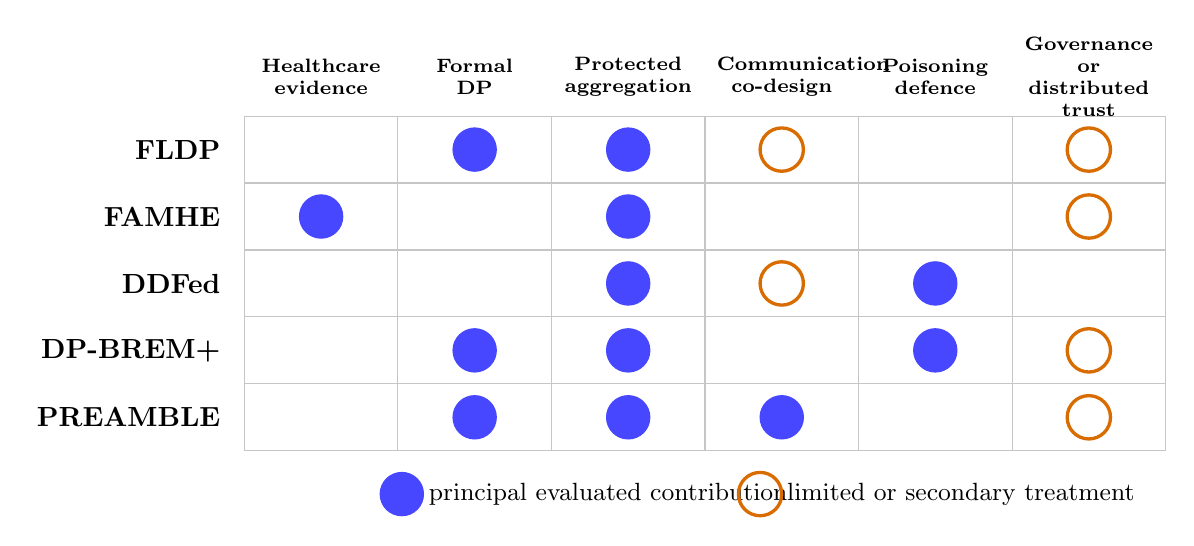
\begin{tikzpicture}[
    font=\small,
    rowlabel/.style={anchor=east, font=\bfseries},
    header/.style={align=center, font=\bfseries\scriptsize, text width=1.65cm},
    strong/.style={circle, fill=blue!72, draw=blue!72, minimum size=5.5mm, inner sep=0pt},
    partial/.style={circle, draw=orange!85!black, line width=1.2pt, minimum size=5.5mm, inner sep=0pt}
]
% grid
\draw[gray!45] (0,0) grid[xstep=1.95,ystep=0.85] (11.7,4.25);
\foreach \x/\name in {
    0.975/{Healthcare\\evidence},
    2.925/{Formal\\DP},
    4.875/{Protected\\aggregation},
    6.825/{Communication\\co-design},
    8.775/{Poisoning\\defence},
    10.725/{Governance or\\distributed trust}}
    \node[header] at (\x,4.75) {\name};

\node[rowlabel] at (-0.18,3.825) {FLDP};
\node[rowlabel] at (-0.18,2.975) {FAMHE};
\node[rowlabel] at (-0.18,2.125) {DDFed};
\node[rowlabel] at (-0.18,1.275) {DP-BREM+};
\node[rowlabel] at (-0.18,0.425) {PREAMBLE};

% FLDP
\node[strong] at (2.925,3.825) {};
\node[strong] at (4.875,3.825) {};
\node[partial] at (6.825,3.825) {};
\node[partial] at (10.725,3.825) {};
% FAMHE
\node[strong] at (0.975,2.975) {};
\node[strong] at (4.875,2.975) {};
\node[partial] at (10.725,2.975) {};
% DDFed
\node[strong] at (4.875,2.125) {};
\node[partial] at (6.825,2.125) {};
\node[strong] at (8.775,2.125) {};
% DP-BREM+
\node[strong] at (2.925,1.275) {};
\node[strong] at (4.875,1.275) {};
\node[strong] at (8.775,1.275) {};
\node[partial] at (10.725,1.275) {};
% PREAMBLE
\node[strong] at (2.925,0.425) {};
\node[strong] at (4.875,0.425) {};
\node[strong] at (6.825,0.425) {};
\node[partial] at (10.725,0.425) {};

\node[strong] at (2.0,-0.55) {};
\node[anchor=west] at (2.22,-0.55) {principal evaluated contribution};
\node[partial] at (6.55,-0.55) {};
\node[anchor=west] at (6.77,-0.55) {limited or secondary treatment};
\end{tikzpicture}%
}
\caption{Capability and assumption map of the five anchor studies. Markers summarize the scope reported in the cited works and should be interpreted with their distinct datasets and threat models.}
\label{fig:anchor-capability-map}
\end{figure}

The anchor studies make the state of the art clearer than a ranking by headline accuracy. FLDP is strongest on efficient malicious-secure private aggregation; FAMHE demonstrates biomedical multiparty cryptography; DDFed and DP-BREM+ integrate privacy with poisoning resistance; and PREAMBLE aligns sparse structure with its cryptographic transport. None evaluates the exact combination of record-level DP, real CKKS serialization, adaptive common-block compression, threshold-governed release, independent aggregate verification, external permissioned audit, and longitudinal clinical poisoning under one frozen protocol.

\subsection{Synthesis of Empirical Studies}

Table~\ref{tab:related-summary} summarizes representative studies without treating their reported metrics as directly exchangeable. Imaging segmentation scores, classification AUROC, private accuracy, attack success, runtime, and communication expansion answer different questions. A fair synthesis therefore records the evaluation unit and the principal missing dimension.

\begin{longtable}{@{}p{2.5cm}p{2.2cm}p{2.8cm}p{3.1cm}p{3.1cm}@{}}
\caption{Representative literature grouped by method and evidence}\label{tab:related-summary}\\
\toprule
Author(s), year & Method & Dataset or setting & Main contribution & Main limitation \\
\midrule
\endfirsthead
\multicolumn{5}{c}{\tablename\ \thetable\ -- continued}\\
\toprule
Author(s), year & Method & Dataset or setting & Main contribution & Main limitation \\
\midrule
\endhead
\bottomrule
\endfoot
McMahan et al., 2017 \cite{mcmahan2017fedavg} & FedAvg & Five non-clinical learning tasks & Established communication-efficient iterative averaging. & No formal privacy, cryptography, or Byzantine defence. \\
Li et al., 2020 \cite{li2020fedprox} & FedProx & Heterogeneous federated benchmarks & Stabilized optimization with a proximal local objective. & Utility method only; result depends on tuning $\mu$. \\
Sheller et al., 2020 \cite{sheller2020federated} & Healthcare FL & Brain-tumour data from 10 institutions & Demonstrated near data-sharing model quality under natural institutional separation. & Did not jointly test DP, HE, poisoning, and communication. \\
Dayan et al., 2021 \cite{dayan2021federated} & EXAM & COVID-19 data from 20 institutions & Demonstrated generalizable multi-site outcome prediction. & Security and cryptographic overhead were not the central evaluation. \\
Ogier du Terrail et al., 2022 \cite{ogier2022flamby} & FLamby benchmark & 7 healthcare datasets, 2--50 silos & Standardized natural healthcare partitions and baselines. & Does not prescribe one privacy or threat model. \\
Stevens et al., 2022 \cite{stevens2022fldp} & FLDP & MNIST, CIFAR-10, synthetic protocol scaling & Combined DP and malicious-secure aggregation efficiently. & No poisoning defence or clinical validation. \\
Li et al., 2022 \cite{li2022soteriafl} & SoteriaFL & Standard FL benchmarks & Unified local DP and shifted compression analysis. & Logical communication is not equivalent to CKKS wire bytes. \\
Li and Li, 2023 \cite{li2023fedef} & Fed-EF & Heterogeneous FL benchmarks & Analyzed error feedback with biased compression. & Stale error under partial participation; no encrypted transport. \\
Xu et al., 2024 \cite{xu2024ddfed} & DDFed & Public cross-device and cross-silo datasets & Coupled FHE privacy with encrypted anomaly detection. & No record-level DP or external governance layer. \\
Gu et al., 2025 \cite{gu2025dpbrem} & DP-BREM/DP-BREM+ & Cross-silo benchmark tasks & Coupled record-level DP and Byzantine robustness, with a secure variant. & No ciphertext-aware adaptive compression or independent ledger. \\
Asi et al., 2025 \cite{asi2025preamble} & PREAMBLE & Private block-sparse vector aggregation & Aligned block sparsity with two-server private aggregation. & Different trust model and no end-to-end healthcare training. \\
\end{longtable}

Across these studies, the literature converges on the need to combine mechanisms. It diverges on the party that is trusted, whether individual updates remain visible, whether compression cost is measured before or after encryption, and whether robustness means a formal bound or success against a finite attack suite. Those differences become the basis for the systematic comparison in the next section.

\section{Comparative Analysis of Existing Approaches}
\label{sec:comparative-analysis}

The comparison uses seven dimensions that are central to this research: predictive utility under heterogeneous hospitals; formal patient privacy; confidentiality of transmitted updates; encrypted communication efficiency; poisoning resistance; decryption and audit governance; and reproducible healthcare evidence. A method receives a qualified rather than absolute assessment because capability depends on assumptions. For example, a coordinate median may be robust when individual updates are visible, but cannot be applied directly when CKKS reveals only their sum.

\begin{table}[htbp]
\centering
\caption{Capability and assumption comparison of principal approaches}
\label{tab:approach-comparison}
\scriptsize
\begin{tabularx}{\textwidth}{@{}p{2.2cm}p{1.45cm}p{1.5cm}p{1.45cm}p{1.45cm}p{1.45cm}p{1.6cm}X@{}}
\toprule
Approach & Non-IID utility & Formal DP & Update confidentiality & Encrypted wire saving & Poisoning defence & Governance/audit & Central assumption or trade-off \\
\midrule
FedAvg/FedProx/SCAFFOLD/FedNova & High, method-dependent & No & No & No & No & No & Optimization baselines; expose updates unless combined with another protocol. \\
DP-FL & Moderate--high, privacy-dependent & Yes & Partial & No & Limited via clipping & No & Noise protects the release, but the server may still see pre-aggregate updates. \\
Secure aggregation/CKKS & Similar to unencrypted arithmetic within approximation & No & Yes & Usually no & No & Key-policy dependent & Hides individual updates but may prevent plaintext anomaly inspection. \\
Logical sparsification/quantization & Method-dependent & No & No & Not guaranteed & No & No & Savings before encryption may disappear after dense re-encoding. \\
Robust plaintext aggregation & Attack-dependent & No & No & No & Yes, under bounds & No & Requires per-client plaintext vectors; may assume a Byzantine limit. \\
FLTrust & Attack-dependent & No & No & No & Yes & Limited & Requires a clean, representative trusted root dataset. \\
FLDP & High within evaluated private tasks & Yes & Yes & Protocol-level reduction & No & Distributed & Efficient malicious-secure private aggregation; no poisoning layer. \\
DDFed & High in reported tasks & No formal DP & Yes & Not primary focus & Yes & Limited & Encrypted anomaly detection under its FHE and anomaly assumptions. \\
DP-BREM+ & High in reported tasks & Yes & Yes & No adaptive scheme & Yes & Distributed & History/momentum plus secure aggregation; no external audit or CKKS-aligned compression. \\
PREAMBLE & Estimation utility & Yes & Yes & Yes, block sparse & No & Two-server & Strong sparse protocol; different task and non-collusion assumption. \\
Proposed hybrid CAABC-FL & Evaluated on natural hospital split & Yes, record-level & Yes, CKKS sum path & Yes, measured from serialized bytes & Empirical validation/reputation gate & Threshold policy, verifier, permissioned ledger & Integrated empirical system; claims remain bounded to evaluated attacks and deployment. \\
\bottomrule
\end{tabularx}
\end{table}

\subsection{Predictive Performance and Generalizability}

FedAvg remains the essential reference because most extensions modify its local training or aggregation path \cite{mcmahan2017fedavg}. FedProx and SCAFFOLD are promising when hospital objectives differ, while FedNova is especially relevant when institutions perform unequal local work \cite{li2020fedprox,karimireddy2020scaffold,wang2020fednova}. No optimizer is uniformly best: its outcome depends on local epochs, client learning rate, participation, feature shift, and label prevalence. The literature therefore supports paired evaluation on the same patient split and seeds rather than importing the best accuracy from separate papers. Centralized and local-only models are also necessary. The centralized model provides a non-private pooled reference, while local-only models show whether collaboration benefits each hospital.

Pooled accuracy alone cannot establish whether a model transfers reliably between hospitals. The natural PhysioNet partition supports three complementary views: combined test performance, performance within each source hospital, and source-to-target transfer. AUROC summarizes ranking across thresholds, whereas AUPRC gives a more informative view of positive-case retrieval when sepsis is uncommon. Calibration and threshold-dependent measures---including sensitivity, specificity, predictive values, F1, balanced accuracy, and Matthews correlation coefficient---describe different operational consequences. To avoid optimistic test estimates, the operating threshold must be chosen from validation predictions and fixed before either pooled or site-specific test outcomes are calculated.

\subsection{Privacy and Security Guarantees}

DP and cryptography answer different questions. DP bounds the influence of a patient on the output distribution \cite{dwork2006calibrating,abadi2016deep}; CKKS or secure aggregation hides a hospital's transmitted update from the server \cite{cheon2017homomorphic,bonawitz2017practical}. Combining them protects both the training transcript and the released model more comprehensively than either mechanism alone. FLDP, DDFed, and DP-BREM+ demonstrate different integration strategies, but their security definitions are not interchangeable \cite{stevens2022fldp,xu2024ddfed,gu2025dpbrem}. FLDP provides malicious-secure private aggregation, DDFed focuses on FHE-protected anomaly detection, and DP-BREM+ couples DP with Byzantine resilience and secure aggregation.

Empirical membership and reconstruction attacks complement, but do not replace, the formal DP statement. Membership AUC near 0.5 can arise from a weak attack, limited sample size, or a genuinely private model. A strong evaluation should therefore report low-false-positive endpoints and uncertainty across independently trained model seeds, guided by modern attacks such as LiRA \cite{carlini2022membership}. Gradient reconstruction should record the attacker's exact visibility, number of optimization steps, reconstruction metric, and success rule \cite{zhu2019dlg,geiping2020inverting}. The same caution applies to cryptography: using CKKS software is not evidence of protocol security unless key ownership, parameter security, message authentication, and decryption policy are specified.

\subsection{Communication and Computational Cost}

Plaintext compressors excel when bandwidth is measured as coordinates or idealized bits. Their advantage can be illusory under HE because every ciphertext carries polynomial data and metadata. Client-specific Top-$k$ also reveals support information unless indices are protected; dense re-encoding hides the support but eliminates wire savings. Common public blocks avoid that contradiction because every hospital packs the same positions. PREAMBLE validates the broader principle that private transport and block sparsity should be designed together \cite{asi2025preamble}, while CAABC-FL applies it to packed CKKS and iterative error feedback.

Communication evaluation should distinguish: (i) logical retained coordinates, (ii) logical encoded bytes, (iii) serialized ciphertext bytes, and (iv) the dense encrypted reference. It should also report encryption, transmission, aggregation, verification, and decryption latency separately. A method that reduces network bytes can still increase total round time through support selection, extra ciphertext operations, or ledger consensus. Conversely, a permissioned ledger may add little bulk to model transport but add a fixed coordination latency. These trade-offs prevent a communication-only result from being described as end-to-end efficiency.

\subsection{Robustness, Availability, and Assumptions}

Plaintext Krum, trimmed mean, coordinate median, RFA, and FLTrust are strong diagnostic baselines, but they operate under visibility or trusted-root assumptions absent from sum-only CKKS \cite{blanchard2017krum,yin2018byzantine,pillutla2022robust,cao2021fltrust}. DDFed reduces this incompatibility through encrypted anomaly processing \cite{xu2024ddfed}. DP-BREM+ uses client history and momentum in a secure aggregation design \cite{gu2025dpbrem}. The proposed validation and reputation gate instead evaluates the candidate global model and can roll back a harmful release. This makes it compatible with an aggregate-only encryption path, but it detects effects rather than inspecting causes.

Robustness must be considered together with availability. A strict rollback rule may prevent a poisoned model from being released while also allowing attackers to halt progress. Reputation can reduce repeated influence, but an adaptive attacker may build trust before activation. Meaningful evaluation therefore includes one-round scaling and sign-flip attacks, backdoors or targeted effects where applicable, collusion, Sybil identities under the identity policy, sleeper attacks, adaptive trust manipulation, and multi-round recovery. Negative results and false rejections should remain visible.

\subsection{Domain Suitability and Resulting Design Choice}

For multi-institutional healthcare, no single reviewed method covers the full requirement set. Optimization-only algorithms are computationally accessible but leave privacy and trust unresolved. Pure DP gives a formal patient-level guarantee but does not hide individual updates from the coordinator. HE hides updates but increases communication and conflicts with plaintext robust aggregation. Blockchain improves accountability but cannot validate the model semantics. Integrated methods such as DDFed and DP-BREM+ are the closest alternatives, yet neither combines ciphertext-aware adaptive block compression, threshold-governed decryption, independent aggregate verification, and an external permissioned audit trail on the target clinical cohort.

The selected design is consequently hybrid. It uses a conventional family of federated optimizers for utility comparison; patient-level clipping, noise, and accounting for formal privacy; CKKS packing for update confidentiality; common adaptive blocks and error feedback for measurable encrypted-wire reduction; validation, rollback, and reputation for empirical poisoning control; threshold authorization to reduce single-custodian key risk; and an independent verifier plus permissioned ledger for accountability. This selection does not imply universal superiority. It is promising because its assumptions match a governed hospital consortium and because its claimed benefits can be tested within one frozen end-to-end protocol.

\section{Summary of Research Gaps}
\label{sec:research-gaps}

The literature review identifies five precise gaps.

\begin{enumerate}
    \item \textbf{Incomplete integration of privacy, communication, robustness, and governance.} Existing work often solves two dimensions well---for example, DP with secure aggregation or FHE with anomaly detection---but fewer systems evaluate all four in one cross-silo clinical workflow \cite{stevens2022fldp,xu2024ddfed,gu2025dpbrem}. The consequence is that a component can invalidate another component's assumption when systems are assembled later.

    \item \textbf{Mismatch between logical compression and encrypted network cost.} Many compression studies report retained coordinates or pre-encryption bits, although sparse supports may require disclosure or dense ciphertext encoding \cite{li2022soteriafl,li2023fedef}. Without serialized-ciphertext measurement, the claimed bandwidth reduction may not exist in the deployed privacy path.

    \item \textbf{Weak alignment between encrypted aggregation and poisoning defence.} Robust rules commonly require individual plaintext updates, while CKKS and secure aggregation intentionally conceal them \cite{blanchard2017krum,yin2018byzantine,bonawitz2017practical}. This creates a privacy--robustness conflict and motivates aggregate-compatible validation, secure anomaly computation, or other independently verifiable controls.

    \item \textbf{Insufficient longitudinal and statistically powered privacy/security evaluation.} One-seed experiments and independent attack trials do not characterize variation between trained models, and one-round attacks omit sleeper, colluding, and adaptive behaviour. Modern membership and reconstruction research further shows that weak average-case attacks can understate leakage \cite{carlini2022membership,geiping2020inverting}. The consequence is overconfident privacy or robustness conclusions.

    \item \textbf{Limited end-to-end key governance and audit evidence.} Threshold HE and permissioned ledgers address custody and traceability, respectively, but a ledger entry alone does not verify aggregation correctness, and a threshold policy alone does not attest custodian behaviour \cite{mouchet2021multiparty,androulaki2018hyperledger}. A practical consortium needs signed authorization, independent verification, model hashes, and externally maintained audit evidence under one protocol.
\end{enumerate}

Table~\ref{tab:gap-objective-map} maps these gaps to the three bachelor-level research objectives. The first objective concerns design, the second implementation, and the third comparative evaluation.

\begin{table}[htbp]
\centering
\caption{Mapping from literature gaps to thesis objectives}
\label{tab:gap-objective-map}
\small
\begin{tabularx}{\textwidth}{@{}p{2.55cm}X X@{}}
\toprule
Research gap & Implication & Thesis objective addressed \\
\midrule
Fragmented protection mechanisms & Independently designed components may expose new trust or data paths when combined. & \textbf{Objective 1:} Design a unified cross-silo architecture combining patient-level DP, CKKS aggregation, communication adaptation, poisoning controls, and governed audit. \\
Logical versus encrypted-cost mismatch & Coordinate sparsity cannot support a network-efficiency claim without ciphertext-aware packing and measurement. & \textbf{Objectives 1 and 2:} Design and implement CAABC-FL with common blocks, error feedback, real CKKS serialization, and explicit transport accounting. \\
Privacy--robustness incompatibility & Plaintext anomaly rules cannot be credited inside a sum-only encrypted path. & \textbf{Objective 2:} Implement an aggregate-compatible validation, rollback, and reputation workflow, alongside independently verified aggregation. \\
Underpowered attack evaluation & Results may be seed-specific and may miss adaptive or low-FPR attacks. & \textbf{Objective 3:} Compare methods with paired seeds, confidence intervals, powered membership inference, long-run reconstruction, and one-round plus longitudinal poisoning. \\
Single-authority and weak audit evidence & A privileged key holder or mutable coordinator log creates a governance bottleneck. & \textbf{Objectives 1 and 2:} Apply threshold-governed decryption, signed authorization, external permissioned logging, and independent transcript verification. \\
\bottomrule
\end{tabularx}
\end{table}

This thesis addresses the most critical gap by evaluating the protection mechanisms as one system rather than presenting them as independent modules. The proposed framework is implemented across authenticated network services and evaluated on a naturally partitioned, full-scale two-hospital PhysioNet cohort. Its comparison includes non-private optimization controls, private and encrypted baselines, logical compression controls, plaintext robust aggregators with their stronger visibility assumptions, and the proposed ciphertext-aligned method. Predictive, calibration, communication, privacy-attack, reconstruction, poisoning, verification, and audit outcomes are analyzed under frozen protocols and paired seeds. The resulting claims remain deliberately bounded: the study evaluates a real multi-service research system under specified attacks and cryptographic settings, but does not claim universal poisoning resistance, universal privacy superiority, a fully decentralized network, or hardware-confidential production deployment. Chapter~3 translates these gaps and boundaries into the conceptual framework, threat model, system architecture, and experimental methodology.
